\chapter{Overenie riešenia}


\section{Využitie pamäte}
\begin{table}[h]
\def\arraystretch{1.25}
\begin{tabular}{|l|llll|lll|}
\hline
                     & \multicolumn{4}{c|}{\textbf{IRAM (192 kB)}}                                                                              & \multicolumn{3}{c|}{\textbf{DRAM (328 kB)}}                                           \\ \hline
\textbf{Sekcia}      & \multicolumn{1}{l|}{CPU cache} & \multicolumn{1}{l|}{.vectors} & \multicolumn{1}{l|}{.text} & voľné                      & \multicolumn{1}{l|}{.bss}  & \multicolumn{1}{l|}{.data} & voľné (heap)                \\ \hline
\textbf{Veľkosť (B)} & \multicolumn{1}{r|}{65536}     & \multicolumn{1}{r|}{1027}     & \multicolumn{1}{r|}{83780} & \multicolumn{1}{r|}{46265} & \multicolumn{1}{r|}{44392} & \multicolumn{1}{r|}{15040} & \multicolumn{1}{r|}{276440} \\ \hline
\end{tabular}
\caption{Rozdelenie pamäte medzi sekcie}
\end{table}

\begin{figure}[h]
	\centering
     \hfill
     \begin{subfigure}{0.48\textwidth}
        \centering
     	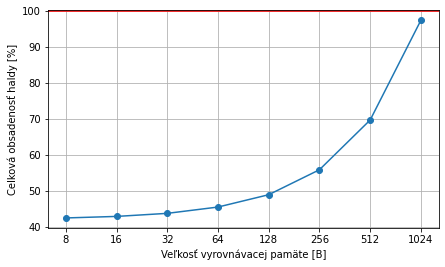
\includegraphics[width=\textwidth]{figures/verification/memory-usage-percentage.png}
     	 \caption{Celková spotreba pamäte}
     \end{subfigure}
     \hfill
      \begin{subfigure}{0.48\textwidth}
    	\centering
        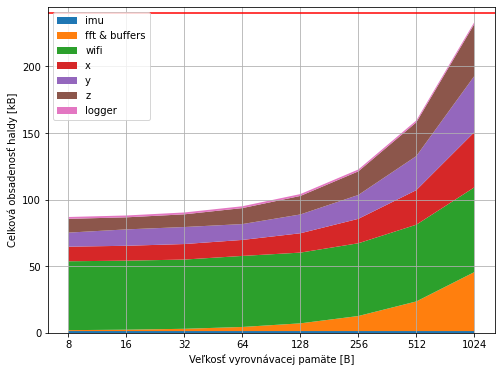
\includegraphics[width=\textwidth]{figures/verification/memory-profile-bytes.png}
         \caption{Rozdelenie pamäte medzi úlohy}
     \end{subfigure}
     \caption{Profilovanie dynamickej pamäte z haldy v DRAM}
\end{figure}

\url{https://blog.espressif.com/esp32-programmers-memory-model-259444d89387}

\section{Veľkosti prenášaných správ cez sieťové spojenie}
Maximálny počet udalostí, aby to bolo efektívne: Parametrická rovnica s parametrom počtom frekvenčných vedierok $m$ 
a počtom udalostí $p$ : $26 + 27 \cdot p < 5 \cdot m$. Percentuálny podiel udalostí: $p / m$. Pre $m = 16$: v priemere 
2 udalosti za okno ($12.5\%$). Pre $m = 512$: v priemere 93 udalostí za okno ($18.16\%$). Výhoda je predspracovanie, 
v tomto prípade aj dosiahneme menší počet prenesených dát. Štatistiky sa oplatí vytvárať pri najmenšom N = 32. $m = n / 2$

\begin{table}[h]
\def\arraystretch{1.25}
\centering
\begin{tabular}{|l|r|r|r|r|r|}
\hline
\textbf{Protokol}         & \textbf{Ethernet II} & \textbf{IPv4} & \textbf{TCP} & \textbf{MQTT}  & \textbf{Spolu}  \\ \hline
\textbf{Veľkosť hlavičky} & 14                   & 20            & 20           & \textgreater 5 & \textgreater 55 \\ \hline
\end{tabular}
\caption{Sieťová réžia}
\end{table}

\begin{table}[h]
\def\arraystretch{1.25}
\centering
\begin{tabular}{|l|r|r|rr|cr|r|l}
\cline{1-8}
\multirow{2}{*}{\textbf{MQTT topic}} & \multicolumn{1}{c|}{\multirow{2}{*}{\textbf{\begin{tabular}[c]{@{}c@{}}Min. \\topic \end{tabular}}}} & \multicolumn{1}{c|}{\multirow{2}{*}{\textbf{\begin{tabular}[c]{@{}c@{}}Veľkosť\\ v RAM\end{tabular}}}} & \multicolumn{2}{l|}{\textbf{Hlavička (h)}}                      & \multicolumn{2}{l|}{\textbf{Prvok (p)}}                         & \multicolumn{1}{c|}{\multirow{2}{*}{\textbf{\begin{tabular}[c]{@{}c@{}}Max. celková\\ veľkosť\end{tabular}}}} & \textbf{} \\ \cline{4-7}
                                     & \multicolumn{1}{c|}{}                                                                                     & \multicolumn{1}{c|}{}                                                                                  & \multicolumn{1}{c|}{\textbf{Min.}} & \multicolumn{1}{c|}{\textbf{Max.}} & \multicolumn{1}{c|}{\textbf{Min.}} & \multicolumn{1}{c|}{\textbf{Max.}} & \multicolumn{1}{c|}{}                                                                                         &           \\ \cline{1-8}
config/response                      & 21                                                                                                        & 124                                                                                                    & \multicolumn{2}{c|}{-}                                                  & \multicolumn{1}{r|}{-}             & \multicolumn{1}{l|}{}              & 450                                                                                                           &           \\ \cline{1-8}
samples                              & 13                                                                                                        & $4\cdot n$                                                                                                    & \multicolumn{1}{r|}{1}             & 3                                  & \multicolumn{2}{c|}{5}                                                  & $h + p\cdot n$                                                                                                      &           \\ \cline{1-8}
spectrum/+                           & 16                                                                                                        & $4\cdot m$                                                                                                & \multicolumn{1}{r|}{14}            & 22                                 & \multicolumn{2}{c|}{5}                                                  & $h + p\cdot m$                                                                                                 &           \\ \cline{1-8}
stats/+                              & 13                                                                                                        & 52                                                                                                     & \multicolumn{1}{r|}{4}             & 8                                  & \multicolumn{1}{r|}{9}             & 12                                 & 127                                                                                                           &           \\ \cline{1-8}
events/+                             & 14                                                                                                        & $20\cdot m$                                                                                               & \multicolumn{1}{r|}{18}            & 26                                 & \multicolumn{1}{r|}{17}            & 27                                 & $h + p\cdot m$                                                                                                &           \\ \cline{1-8}
\end{tabular}
\caption{Veľkosti správ pre MQTT topics}
\end{table}



\section{Čas vykonávania algoritmov}

\begin{table}[h]
\def\arraystretch{1.25}
\centering
\begin{tabular}{|l|l|l|l|l|l|l|}
\hline
\textbf{Veľkosť okna}         & \textbf{32} & \textbf{64} & \textbf{128} & \textbf{256} & \textbf{512} & \textbf{1024} \\ \hline
\textbf{Štatistiky bez korelácii}& 3673        & 7471        & 14652        & 29574        & 59158        & 112871        \\ \hline
\textbf{DFT}                     & 80          & 162         & 306          & 611          & 1243         & 2620          \\ \hline
\textbf{DCT}                     & 91          & 165         & 310          & 612          & 1226         & 2532          \\ \hline
\textbf{Špičky: susedia}         & 45          & 102         & 216          & 451          & 913          & 1812          \\ \hline
\textbf{Špičky: nulou do záporu} & 6           & 10          & 17           & 33           & 62           & 121           \\ \hline
\textbf{Špičky: horský turista}  & 19          & 32          & 54           & 109          & 199          & 431           \\ \hline
\textbf{Udalosti}                & 7           & 10          & 17           & 31           & 58           & 114           \\ \hline
\end{tabular}
\caption{Čas vykonávania algoritmov od veľkosti vyrovnávacej pamäte v mikrosekundách pri taktovacej frekvencii 80 MHz a preemtívnom
ticku 100 Hz}
\end{table}

\begin{table}[h]
\def\arraystretch{1.25}
\centering
\begin{tabular}{|l|r|r|r|}
\hline
\textbf{Veľkosť masky}  & \textbf{4} & \textbf{16} & \textbf{64} \\ \hline
\textbf{1x} & 108        & 262         & 891         \\ \hline
\textbf{4x} & 413        & 1041        & 3697        \\ \hline
\textbf{8x} & 819        & 2065        & 7209        \\ \hline
\end{tabular}
\caption{Čas v mikrosekundách na vyhladzovanie frekvenčného spektra v závislosti od veľkosti konvolučného jadra pri N = 512 a počtu opakovaných prechodov}
\end{table}


\section{Čas vykonávania pipeline}
Hraničný čas na dokončenie úlohy v reálnom čase v sekundách pre jednu vyrovnávaciu pamäť je $t \leq n / f_s$.
Podľa parametrickej nerovnice vieme určiť pre akú vzorkovaciu frekvenciu pri danej veľkosti okna je prekročená stanovená hranica:
$ f_s < n / t $. Všetky spracovania prebehnú do limitu zatiaľ čo sa zbiera druhé okno vzoriek. 

Hraničná najvyššia vzorkovacia pre double-buffer je pre jednu os spracovania 61,776 kHz a 12,785 kHz pre 3 osi spracovania.
Pre posielanie štatistík a spektra je max. vzorkovacia frekevencia 2,1 KHz, ale pri vyšších bufferoch sa pohybuje nad 7 KHz.
Pri 3 osiach spracovania je to max. 1320 Hz (N=32), 2510 Hz (N=256), 3741 Hz (N=1024)

\begin{table*}[h]
     \def\arraystretch{1.25}
	 \centering
     \captionsetup[subtable]{position=below}
     \captionsetup[table]{position=below}
     \caption{Čas na spracovanie okna vzoriek v mikrosekundách.}
     
     \begin{subtable}{0.48\linewidth}
         \centering
		\begin{tabular}{|l|l|r|r|r|}
		\hline
		\textbf{}                       & \textbf{N}  & \textbf{32} & \textbf{256} & \textbf{1024} \\ \hline
		\multirow{3}{*}{\textbf{1 os}}  & \textbf{A1} & 518         & 2616         & 6401          \\ \cline{2-5} 
 		                                & \textbf{A2} & 435         & 1598         & 6209          \\ \cline{2-5} 
                                        & \textbf{A3} & 467         & 1695         & 3864          \\ \hline
		\multirow{3}{*}{\textbf{3 osi}} & \textbf{A1} & 2503        & 3077         & 10177         \\ \cline{2-5} 
                                        & \textbf{A2} & 556         & 3340         & 10334         \\ \cline{2-5} 
                                        & \textbf{A3} & 591         & 1295         & 4670          \\ \hline
		\end{tabular}
		\caption{Čas na spracovanie okna vzoriek v mikrosekundách. Zariadenie v pokoji bez spracovania štatistík. FFT}
	\end{subtable}
    \hfill
    \begin{subtable}{0.48\linewidth}
         \centering
		\begin{tabular}{|l|l|r|r|r|}
		\hline
		\textbf{}                       & \textbf{N}  & \textbf{32} & \textbf{256} & \textbf{1024} \\ \hline
		\multirow{3}{*}{\textbf{1 os}}  & \textbf{A1} & 14750       & 34883        & 129190        \\ \cline{2-5} 
                              			& \textbf{A2} & 8824        & 34351        & 139451        \\ \cline{2-5} 
                                        & \textbf{A3} & 13795       & 34890        & 137346        \\ \hline
		\multirow{3}{*}{\textbf{3 osi}} & \textbf{A1} & 23851       & 101978       & 273696        \\ \cline{2-5} 
                                        & \textbf{A2} & 22981       & 78972        & 272161        \\ \cline{2-5} 
                                        & \textbf{A3} & 24232       & 100156       & 270110        \\ \hline
		\end{tabular}
		\caption{Priemer z maxima z časov potrebných na spracovanie okna ktorejkoľvek osi spracovania. Posielanie štatistík s koreláciou           a frekvenčného spektra s FFT. RSSI je približne -40}
	\end{subtable}
\end{table*}

\section{Jednotkové testy na konzistenciu C a Python verzii}


\section{Úspešnosť algoritmov na detekciu špičiek}

Prevalencia javu - počet špičiek v okne (8 pri 238, 16 pri 476, 32 pri 952) 
Generovanie frekvencií sinusoíd s exponenciálnymi fade-in/out o dĺžke desatiny trvania, aby sa znížili hraničné javy vo frekvenčnom spektre. S pevným počtom komponentov posunutým v čase a trvaním v počte dielikov a podkladový normálne rozdelený šum.
Vytvorenie testovacom signále s trvaním 60 sekúnd
so seedom 10 a následne trénovacom signále s trvaním 20 sekúnd. Na trénovacom signále sa vyberú najlepšie parametre
vrámci prehľadávaného priestoru cez grid search. Vyhodnotenie metrík prebieha na testovacom signále v porovnaní s predpisom.
Stanovenie parametrov je nepresné, vyžaduje sa manuálne adaptovať hyperparametre podľa situácie. Na ilustráciu
sú presnosti a parametre v tabuľkách, dá sa použiť ako referencia pre výhodný rozsah hodnôt. FFT s prekryvom 50\% a Hannovo okno

Relevantná metriky. Vysoká fs zároveň s nízkym n dávajú nižšie presnosti.

\begin{table}[h]
\def\arraystretch{1.1}
\centering
\begin{tabular}{|c|ccc|ccc|ccc|}
\hline
                    & \multicolumn{3}{c|}{\textbf{Algoritmus 1}}                                           & \multicolumn{3}{c|}{\textbf{Algoritmus 2}}                                           & \multicolumn{3}{c|}{\textbf{Algoritmus 3}}                                           \\ \hline
\diagbox{$n$}{$f_s$} & \multicolumn{1}{c|}{\textbf{238}} & \multicolumn{1}{c|}{\textbf{476}} & \textbf{952} & \multicolumn{1}{c|}{\textbf{238}} & \multicolumn{1}{c|}{\textbf{476}} & \textbf{952} & \multicolumn{1}{c|}{\textbf{238}} & \multicolumn{1}{c|}{\textbf{476}} & \textbf{952} \\ \hline
\textbf{128}        & \multicolumn{1}{c|}{84.46}        & \multicolumn{1}{c|}{73.76}        & 59.49        & \multicolumn{1}{c|}{83.67}        & \multicolumn{1}{c|}{74.12}        & 54.96        & \multicolumn{1}{c|}{83.69}        & \multicolumn{1}{c|}{73.41}        & 51.87        \\ \hline
\textbf{256}        & \multicolumn{1}{c|}{91.19}        & \multicolumn{1}{c|}{85.41}        & 73.59        & \multicolumn{1}{c|}{90.63}        & \multicolumn{1}{c|}{84.39}        & 71.84        & \multicolumn{1}{c|}{91.30}        & \multicolumn{1}{c|}{84.78}        & 72.00        \\ \hline
\textbf{512}        & \multicolumn{1}{c|}{95.54}        & \multicolumn{1}{c|}{91.91}        & 85.19        & \multicolumn{1}{c|}{95.45}        & \multicolumn{1}{c|}{91.92}        & 84.05        & \multicolumn{1}{c|}{95.54}        & \multicolumn{1}{c|}{91.93}        & 85.05        \\ \hline
\end{tabular}
\caption{Presnosť v percentách}
\end{table}

\begin{table}[h]
\def\arraystretch{1.1}
\centering
\begin{tabular}{|c|lll|lll|lll|}
\hline
                    & \multicolumn{3}{c|}{\textbf{Algoritmus 1}}                                                                & \multicolumn{3}{c|}{\textbf{Algoritmus 2}}                                                                & \multicolumn{3}{c|}{\textbf{Algoritmus 3}}                                                                \\ \hline
\diagbox{$n$}{$f_s$}  & \multicolumn{1}{c|}{\textbf{238}} & \multicolumn{1}{c|}{\textbf{476}} & \multicolumn{1}{c|}{\textbf{952}} & \multicolumn{1}{c|}{\textbf{238}} & \multicolumn{1}{c|}{\textbf{476}} & \multicolumn{1}{c|}{\textbf{952}} & \multicolumn{1}{c|}{\textbf{238}} & \multicolumn{1}{c|}{\textbf{476}} & \multicolumn{1}{c|}{\textbf{952}} \\ \hline
\textbf{128}        & \multicolumn{1}{l|}{23.77}        & \multicolumn{1}{l|}{35.52}        & 41.04                             & \multicolumn{1}{l|}{16.11}        & \multicolumn{1}{l|}{22.33}        & 21.94                             & \multicolumn{1}{l|}{9.65}         & \multicolumn{1}{l|}{14.58}        & 9.47                              \\ \hline
\textbf{256}        & \multicolumn{1}{l|}{10.62}        & \multicolumn{1}{l|}{27.42}        & 29.98                             & \multicolumn{1}{l|}{6.58}         & \multicolumn{1}{l|}{15.33}        & 28.03                             & \multicolumn{1}{l|}{13.26}        & \multicolumn{1}{l|}{11.88}        & 9.51                              \\ \hline
\textbf{512}        & \multicolumn{1}{l|}{12.08}        & \multicolumn{1}{l|}{14.52}        & 32.09                             & \multicolumn{1}{l|}{3.68}         & \multicolumn{1}{l|}{0.00}         & 17.13                             & \multicolumn{1}{l|}{2.35}         & \multicolumn{1}{l|}{1.80}         & 15.26                             \\ \hline
\end{tabular}
\caption{TPR - True positive rate (Senzitivita)}
\end{table}

\begin{table}[h]
\def\arraystretch{1.1}
\centering
\begin{tabular}{|c|lll|lll|lll|}
\hline
                    & \multicolumn{3}{c|}{\textbf{Algoritmus 1}}                                                                & \multicolumn{3}{c|}{\textbf{Algoritmus 2}}                                                                & \multicolumn{3}{c|}{\textbf{Algoritmus 3}}                                                                \\ \hline
\diagbox{$n$}{$f_s$} & \multicolumn{1}{c|}{\textbf{238}} & \multicolumn{1}{c|}{\textbf{476}} & \multicolumn{1}{c|}{\textbf{952}} & \multicolumn{1}{c|}{\textbf{238}} & \multicolumn{1}{c|}{\textbf{476}} & \multicolumn{1}{c|}{\textbf{952}} & \multicolumn{1}{c|}{\textbf{238}} & \multicolumn{1}{c|}{\textbf{476}} & \multicolumn{1}{c|}{\textbf{952}} \\ \hline
\textbf{128}        & \multicolumn{1}{l|}{3.67}         & \multicolumn{1}{l|}{11.31}        & 21.59                             & \multicolumn{1}{l|}{3.06}         & \multicolumn{1}{l|}{5.38}         & 11.38                             & \multicolumn{1}{l|}{1.75}         & \multicolumn{1}{l|}{3.36}         & 4.87                              \\ \hline
\textbf{256}        & \multicolumn{1}{l|}{1.08}         & \multicolumn{1}{l|}{4.10}         & 8.66                              & \multicolumn{1}{l|}{1.26}         & \multicolumn{1}{l|}{3.12}         & 10.33                             & \multicolumn{1}{l|}{1.19}         & \multicolumn{1}{l|}{1.97}         & 2.41                              \\ \hline
\textbf{512}        & \multicolumn{1}{l|}{5.27}         & \multicolumn{1}{l|}{1.30}         & 5.00                              & \multicolumn{1}{l|}{0.96}         & \multicolumn{1}{l|}{0.00}         & 3.48                              & \multicolumn{1}{l|}{0.96}         & \multicolumn{1}{l|}{0.15}         & 1.95                              \\ \hline
\end{tabular}
\caption{FPR - False positive rate (Chybovosť)}
\end{table}


\begin{table}[h]
\def\arraystretch{1.1}
\centering
\begin{tabular}{|c|c|ccc|cc|cccc|}
\hline
\multirow{2}{*}{\textbf{\begin{tabular}[c]{@{}c@{}}$f_s$\end{tabular}}} & \multirow{2}{*}{\textbf{\begin{tabular}[c]{@{}c@{}}$n$\end{tabular}}} & \multicolumn{3}{c|}{\textbf{\begin{tabular}[c]{@{}c@{}}A1: Najvyšší \\ spomedzi  susedov\end{tabular}}} & \multicolumn{2}{c|}{\textbf{\begin{tabular}[c]{@{}c@{}}A2: Prechod\\ nulou do záporu\end{tabular}}} & \multicolumn{4}{c|}{\textbf{\begin{tabular}[c]{@{}c@{}}A3: Horský\\ turista\end{tabular}}}  \\ \cline{3-11} 
                                                                                  &                                                                         & \multicolumn{1}{c|}{\hspace*{3mm}$k$\hspace*{3mm}}         & \multicolumn{1}{c|}{\hspace*{3mm}$\epsilon$\hspace*{3mm}}         & $h_{rel}$       & \multicolumn{1}{c|}{\hspace*{4mm} $k$ \hspace*{4mm}}                               &  $s$                              & \multicolumn{1}{c|}{$t$} & \multicolumn{1}{c|}{$h$} & \multicolumn{1}{c|}{$p$} & $i$ \\ \hline
238                                                                               & 128                                                                     & \multicolumn{1}{c|}{12}          & \multicolumn{1}{c|}{3}                  & 32                & \multicolumn{1}{c|}{2}                                 & 12                                & \multicolumn{1}{c|}{16}  & \multicolumn{1}{c|}{0}   & \multicolumn{1}{c|}{10}  & 8   \\ \hline
238                                                                               & 256                                                                     & \multicolumn{1}{c|}{3}           & \multicolumn{1}{c|}{1}                  & 32                & \multicolumn{1}{c|}{2}                                 & 16                                & \multicolumn{1}{c|}{16}  & \multicolumn{1}{c|}{0}   & \multicolumn{1}{c|}{10}  & 12  \\ \hline
238                                                                               & 512                                                                     & \multicolumn{1}{c|}{3}           & \multicolumn{1}{c|}{4}                  & 32                & \multicolumn{1}{c|}{2}                                 & 26                                & \multicolumn{1}{c|}{10}  & \multicolumn{1}{c|}{4}   & \multicolumn{1}{c|}{38}  & 0   \\ \hline
476                                                                               & 128                                                                     & \multicolumn{1}{c|}{3}           & \multicolumn{1}{c|}{4}                  & 16                & \multicolumn{1}{c|}{2}                                 & 9                                 & \multicolumn{1}{c|}{10}  & \multicolumn{1}{c|}{0}   & \multicolumn{1}{c|}{10}  & 0   \\ \hline
476                                                                               & 256                                                                     & \multicolumn{1}{c|}{12}          & \multicolumn{1}{c|}{4}                  & 32                & \multicolumn{1}{c|}{2}                                 & 12                                & \multicolumn{1}{c|}{16}  & \multicolumn{1}{c|}{0}   & \multicolumn{1}{c|}{10}  & 0   \\ \hline
476                                                                               & 512                                                                     & \multicolumn{1}{c|}{3}           & \multicolumn{1}{c|}{4}                  & 32                & \multicolumn{1}{c|}{1}                                 & 20                                & \multicolumn{1}{c|}{10}  & \multicolumn{1}{c|}{4}   & \multicolumn{1}{c|}{33}  & 0   \\ \hline
952                                                                               & 128                                                                     & \multicolumn{1}{c|}{3}           & \multicolumn{1}{c|}{4}                  & 0                 & \multicolumn{1}{c|}{2}                                 & 5                                 & \multicolumn{1}{c|}{10}  & \multicolumn{1}{c|}{0}   & \multicolumn{1}{c|}{10}  & 0   \\ \hline
952                                                                               & 256                                                                     & \multicolumn{1}{c|}{6}           & \multicolumn{1}{c|}{4}                  & 24                & \multicolumn{1}{c|}{2}                                 & 5                                 & \multicolumn{1}{c|}{16}  & \multicolumn{1}{c|}{0}   & \multicolumn{1}{c|}{10}  & 0   \\ \hline
952                                                                               & 512                                                                     & \multicolumn{1}{c|}{6}           & \multicolumn{1}{c|}{4}                  & 32                & \multicolumn{1}{c|}{2}                                 & 12                                & \multicolumn{1}{c|}{16}  & \multicolumn{1}{c|}{0}   & \multicolumn{1}{c|}{10}  & 0   \\ \hline
\end{tabular}
\caption{Parametre algoritmov z grid search detekcie špičiek na syntetických dátach}
\end{table}


% Best parametre algoritmu z grid search

\section{Spektrá a eventy v syntetických dátach}
\begin{figure}[h]
	\centering
     \begin{subfigure}{\textwidth}
        \centering
     	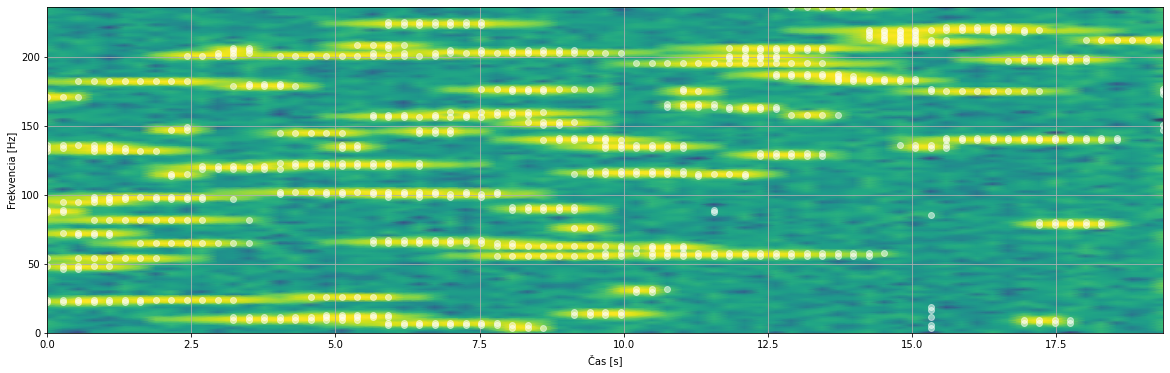
\includegraphics[width=\textwidth]{figures/verification/Sythetic-FFT-A1-476-256.png}
     	\caption{Algoritmus č.1}
     \end{subfigure}
     \begin{subfigure}{\textwidth}
    	\centering
        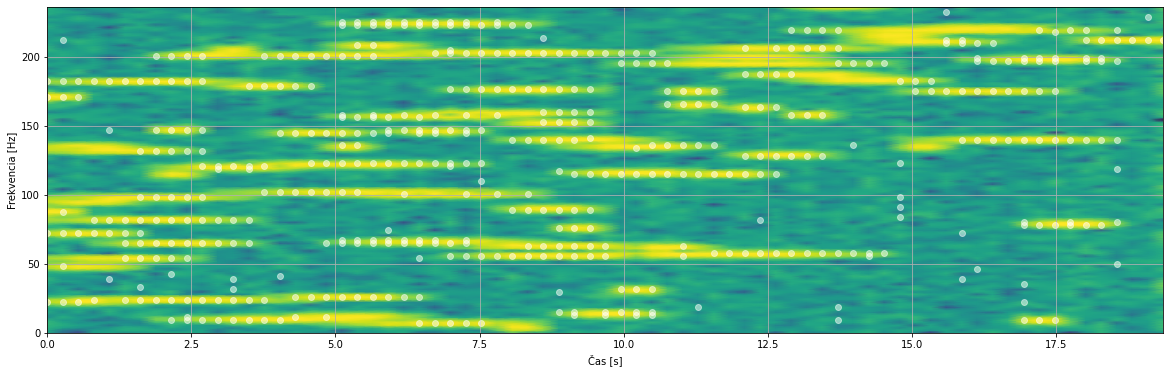
\includegraphics[width=\textwidth]{figures/verification/Sythetic-FFT-A2-476-256.png}
        \caption{Algoritmus č.2}
     \end{subfigure}
      \begin{subfigure}{\textwidth}
    	\centering
        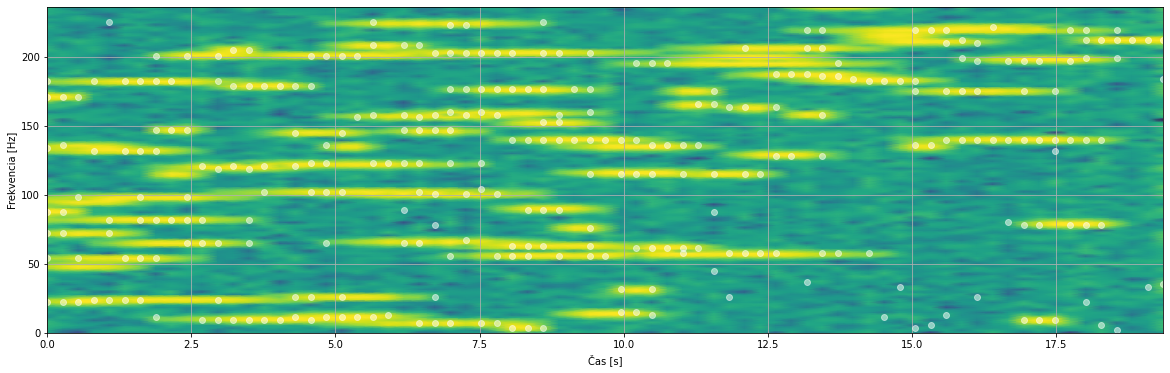
\includegraphics[width=\textwidth]{figures/verification/Sythetic-FFT-A3-476-256.png}
        \caption{Algoritmus č.3}
     \end{subfigure}     
     \caption{Ilustrácia detegovaných špičiek pri fs 476Hz a N = 256 a parametrov podľa grid search}
\end{figure}

\begin{figure}[h]
   \centering
    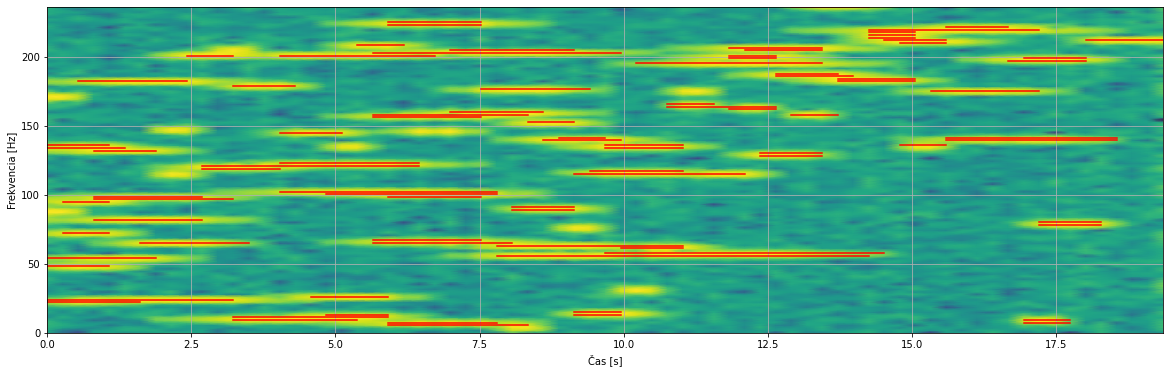
\includegraphics[width=\textwidth]{figures/verification/Sythetic-A1-events.png}
   \caption{Algoritmus č.1 a detekcia udalostí min duration = 4 a time proximity = 1}
\end{figure}  



\section{Obrázky spektier z reálnych datasetov}
Popis datasetov - vzorkovacia frekvencia 500 Hz mestská hromadná doprava (autobusy a električky) na suchých nových cestách.

\begin{figure}[h]
   \centering
    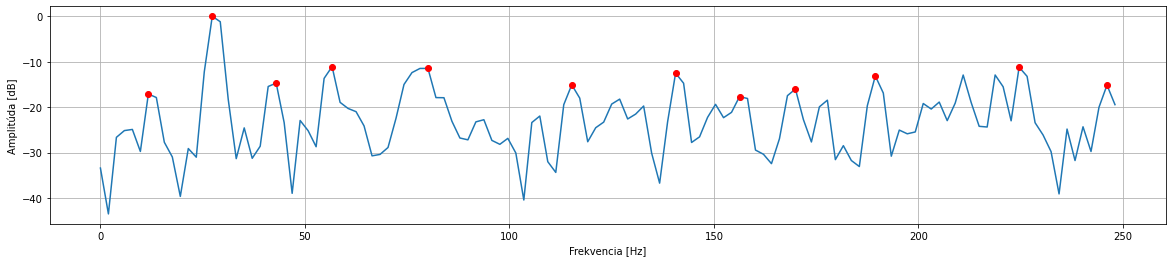
\includegraphics[width=\textwidth]{figures/verification/L83-slice-t-20-A1.png}
   \caption{Prierez spektrogramu. Frekvenčná transformácia okna v 20. sekunde s detegovanými špičkami algoritmom č.1. Je patrné, že
   niektoré vrcholy sú ignorované - zložité odlíšiť šum od signálu. V lineárnej mierke by sme ťažko určovali význačnosť vrchola}
\end{figure} 


\begin{figure}[h]
	\centering
     \begin{subfigure}{\textwidth}
        \centering
     	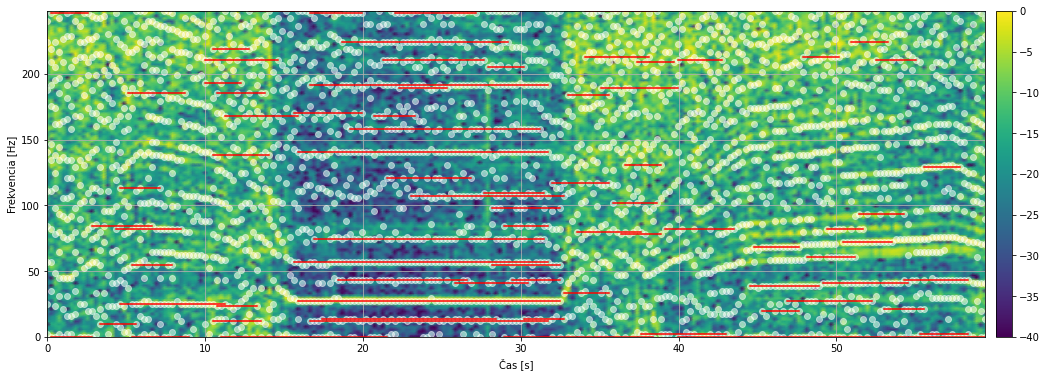
\includegraphics[width=\textwidth]{figures/verification/L83-dataset-A1.png}
     	\caption{Algoritmus č.1}
     \end{subfigure}
     \begin{subfigure}{\textwidth}
    	\centering
        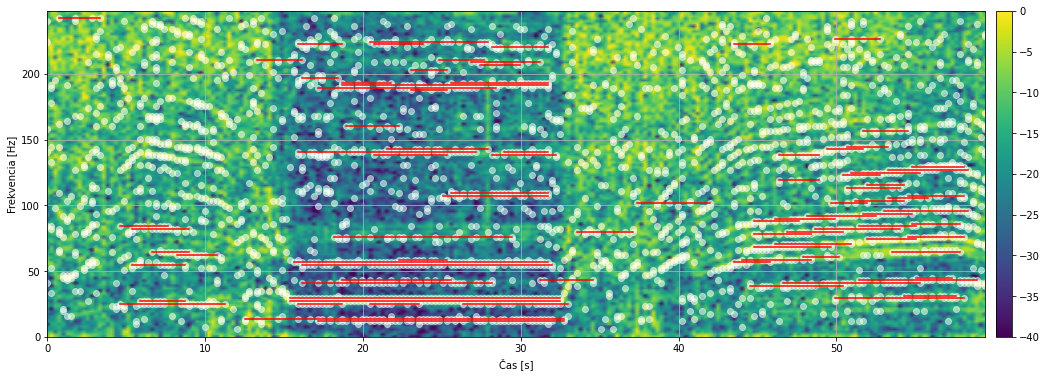
\includegraphics[width=\textwidth]{figures/verification/L83-dataset-A2.png}
        \caption{Algoritmus č.2}
     \end{subfigure}
      \begin{subfigure}{\textwidth}
    	\centering
        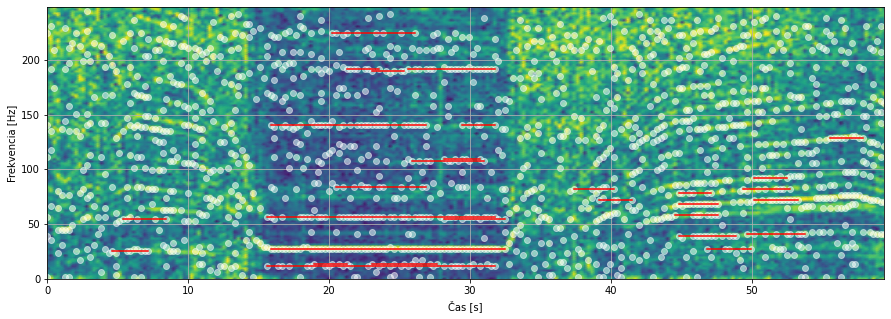
\includegraphics[width=\textwidth]{figures/verification/L83-dataset-A3.png}
        \caption{Algoritmus č.3}
     \end{subfigure}     
     \caption{L83 - Ilustrácia detegovaných špičiek pri fs 476Hz a N = 256 a parametrov podľa grid search}
\end{figure}

\emptypage
